\chapter{Mengenal Python dan Anaconda}
Tujuan pembelajaran pada pertemuan pertama antara lain:
\begin{enumerate}
\item
Mengerti sejarah python, perkembangan dan penggunaan python di perusahaan
\item
Memahami tahapan instalasi python dan anaconda
\item
Memahami cara penggunaan spyder
\end{enumerate}
Tugas dengan cara dikumpulkan dengan pull request ke github dengan menggunakan format latex pada repo yang dibuat oleh asisten IRC.

\section{Teori}
Praktek teori penunjang yang dikerjakan :
\begin{enumerate}
\item
Buat Resume Sejarah Python, perbedaan python 2 dan 3, dengan bahasa yang mudah dipahami dan dimengerti. Buatan sendiri bebas plagiat(10)
\item
Buat Resume Implementasi dan penggunaan Python di perusahaan dunia, bahasa yang mudah dipahami(10)
\end{enumerate}

\section{Instalasi}
Melakukan instalasi python dan anaconda versi 3 serta uji coba spyder. Dengan menggunakan bahasa yang mudah dimengerti dan bebas plagiat. 
Dan wajib skrinsut dari komputer sendiri.
\begin{enumerate}
\item
Instalasi python 3 (5)
\item
instalasi pip(5)
\item
cara setting environment (5)
\item
mencoba entrepreter/cli melakui terminal atau cmd windows(5)
\item 
Menjalankan dan mengupdate anaconda dan spyder(5)
\item
Cara menjalankan Script hello word di spyder(5)
\item
Cara menjalankan Script otomatis login aplikasi akademik dengan library selenium dan inputan user(5)
\item
Cara pemakaian variable explorer di spyder(5)
\end{enumerate}


\section{Identasi}
Membuat file main.py dan mengisinya dengan script contoh python penggunaan selenium(minimal 20 baris) yang melibatkan inputan user, kemudian mencoba untuk mengatasi error identasi.
\begin{enumerate}
	\item
Penjelasan Identasi (10)
	\item
jenis jenis error identasi yang didapat(10)
\item
cara membaca error(10)
\item 
cara menangani errornya(10)
\end{enumerate}

\section{Presentasi Tugas}
Pada pertemuan ini, diadakan tiga penilaiain yaitu penilaian untuk tugas mingguan dengan nilai maksimal 100. Kemudian dalam satu minggu kedepan maksimal sebelum waktu mata kuliah. Ada presentasi kematerian dengan nilai presentasi yang terpisah masing-masing 100. Dan nilai terpisah untuk tutorial dari jawaban tugas di YouTube.Jadi ada tiga komponen penilaiain pada pertemuan ini yaitu :
\begin{enumerate}
	\item tugas minggu hari ini dan besok (maks 100). pada chapter ini
	\item presentasi csv (maks 100). Mempraktekkan kode python dan menjelaskan cara kerjanya.
	\item pembuatan video tutorial youtube tentang tutorial dari jawaban tugas.(nilai maks 100)
\end{enumerate}
Waktu presentasi pada jam kerja di IRC. Kriteria penilaian presentasi sangat sederhana, presenter akan ditanyai 20(10 pertanyaan program, 10 pertanyaan teori) pertanyaan tentang pemahamannya menggunakan python dan program agan dibuat error hingga presenter bisa menyelesaikan errornya. jika presenter tidak bisa menjawab satu pertanyaan asisten maka nilai nol. Jika semua pertanyaan bisa dijawab maka nilai 100. Presentasi bisa diulang apabila gagal, sampai bisa mendapatkan nilai 100 dalam waktu satu minggu kedepan.
\item\textbf{Jawaban Chapter 1}
\begin{enumerate}
\item Python adalah Bahasa pemrograman kelanjutan dari Bahasa pemrograman ABC python pada  Versi terakhir 1.2. yang dikeluarkan oleh CWI yang dikembangkan oleh Guido van Rossum pada tahun 1990 di CWI.Nama Python diciptakan oleh Guino karena pada saat itu Guino cinta pada acara televisi Monty Python s Flying Circus.
\par
Pada tahun 1995, Guido pindah ke CNRI dan mengembangkan pyhton pada tahun 2000 yaitu versi 1.6. Setelah itu Guido dan para pengembang inti pindah ke BeOpen.com berupa perusahaan komersial dan membentuk beOpen PyhtonLabs yang mengeluarkan Pyhton 2.0 dan beberapa dari anggota tim PyhtonLabs pindah ke DigitalCreations
\par
Sekarang pengembangan pyhton dilakukan oleh programmer yang dikoordinir oleh Guido dan Pyhton Software Foundation. Python Software Foundation adalah organisasi non-profit yang dibentuk untuk memegang hak cipta intelektual. Pada sejak python versi 2.1 mencegah pyhton dimiliki oleh perusahaan komersial.Saat ini pyhton telah mencapai 2.6.1 dan versi 3.0
\par
Adapun perbedaan pada pyhton 2 dan 3 yaitu : Syntax untuk mencetak teks atau yang lainnya, Syntax untuk meminta inputan dan hasil dari operator pembagian.

    \item Banyak penggunaan Bahasa pemrograman pyhton dalam sehari hari contohnya pada penerapan pyhton dalam analisis data, menampilkan timline, data scientist dll. Perusahaan yang telah menggunakan pyhton adalah google,youtube,facebook
    ,Instagram,pinterest,dropbox,quora dll.
\end{enumerate}
\textbf{Instalasi}
\begin{enumerate}
\item Instalasi pyhton 3
\begin{itemize}
    \item jalankan aplikasi untuk menginstal dan centang add python lalu klik install now 1.1
    \begin{figure}
        \centering
        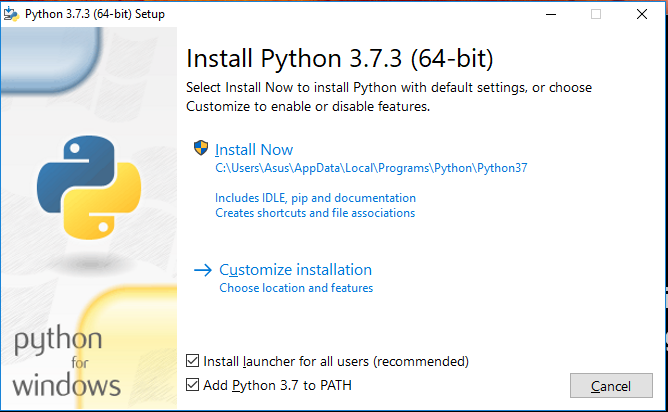
\includegraphics[scale=0.5]{figures/1.PNG}
        \caption{Caption}
        \label{fig:my_label}
    \end{figure}
    \item Lalu tunggu proses installasi 1.2
    \begin{figure}
        \centering
        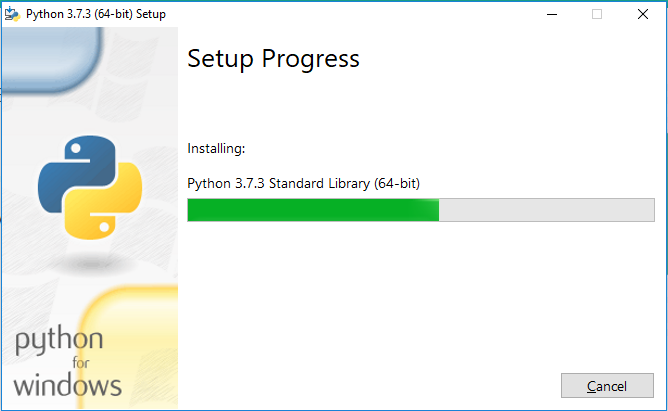
\includegraphics[scale=0.5]{figures/2.PNG}
        \caption{Caption}
        \label{fig:my_label}
    \end{figure}
    \item installasi selesai 1.3
    \begin{figure}
        \centering
        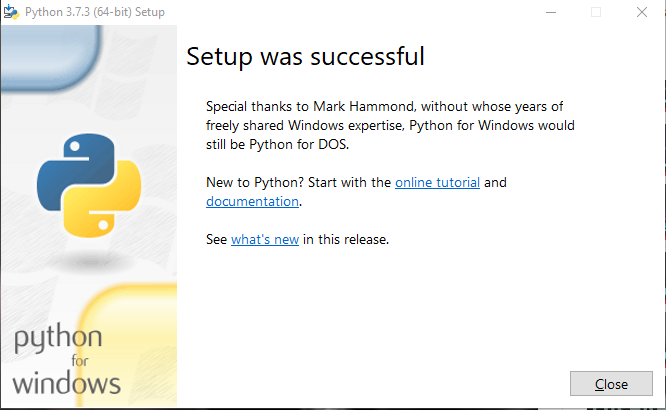
\includegraphics[scale=0.5]{figures/3.PNG}
        \caption{Caption}
        \label{fig:my_label}
    \end{figure}
\end{itemize}
    \item Instalasi PIP
    \begin{itemize}
    \item buka link PIP https://pip.pypa.io/en/stable/installing/ lalu save link yang get-pip.py 1.4
    \begin{figure}
        \centering
        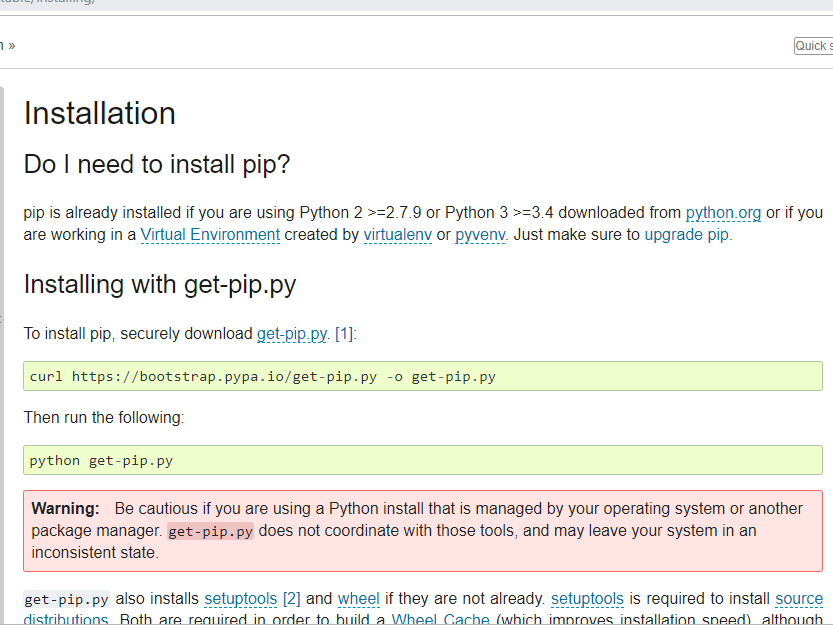
\includegraphics[scale=0.5]{figures/4 (2).PNG}
        \caption{Caption}
        \label{fig:my_label}
    \end{figure}
        \item lalu buka file link yang tadi dengan open with pyhton 1.5 
        \begin{figure}
            \centering
            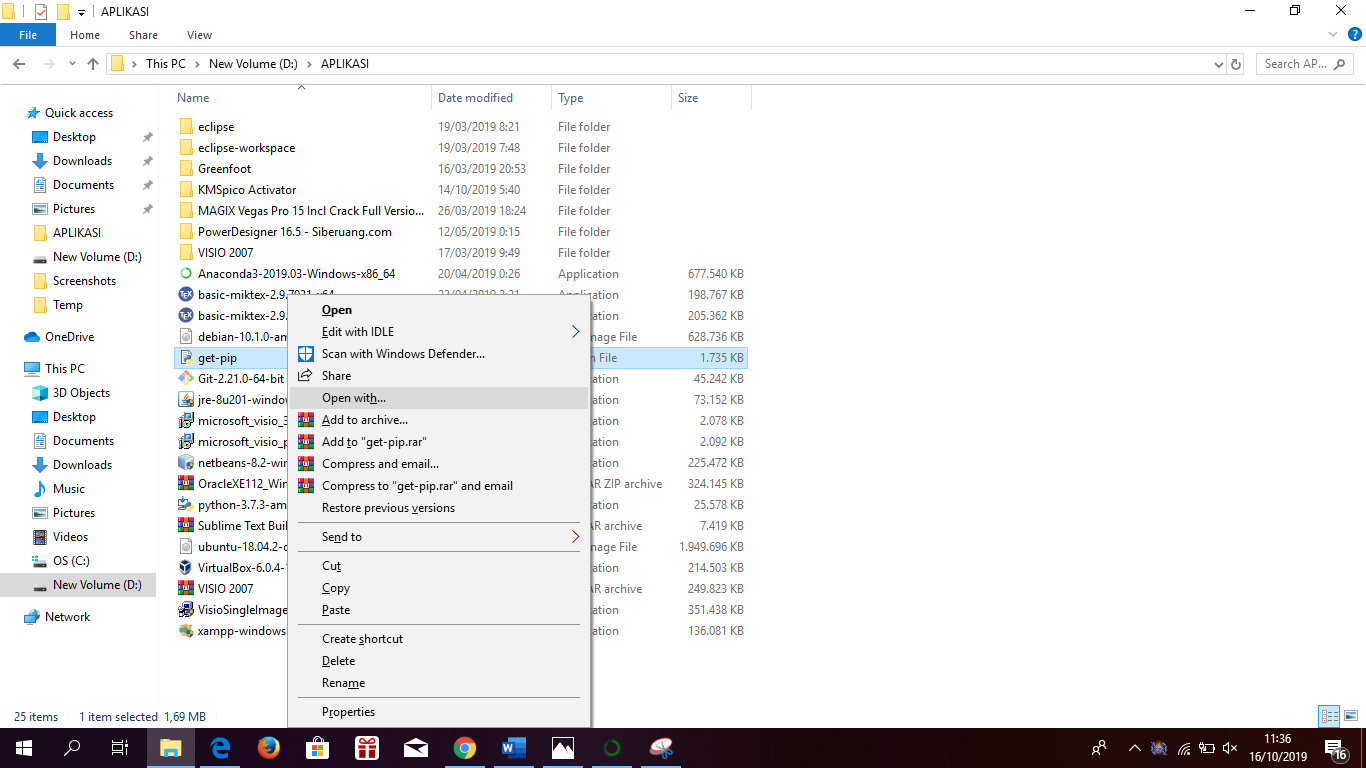
\includegraphics[scale=0.5]{figures/Screenshot (16).png}
            \caption{Caption}
            \label{fig:my_label}
        \end{figure}
        \item setelah dibuka tunggu sampai selesai 1.6
        \begin{figure}
        \centering
        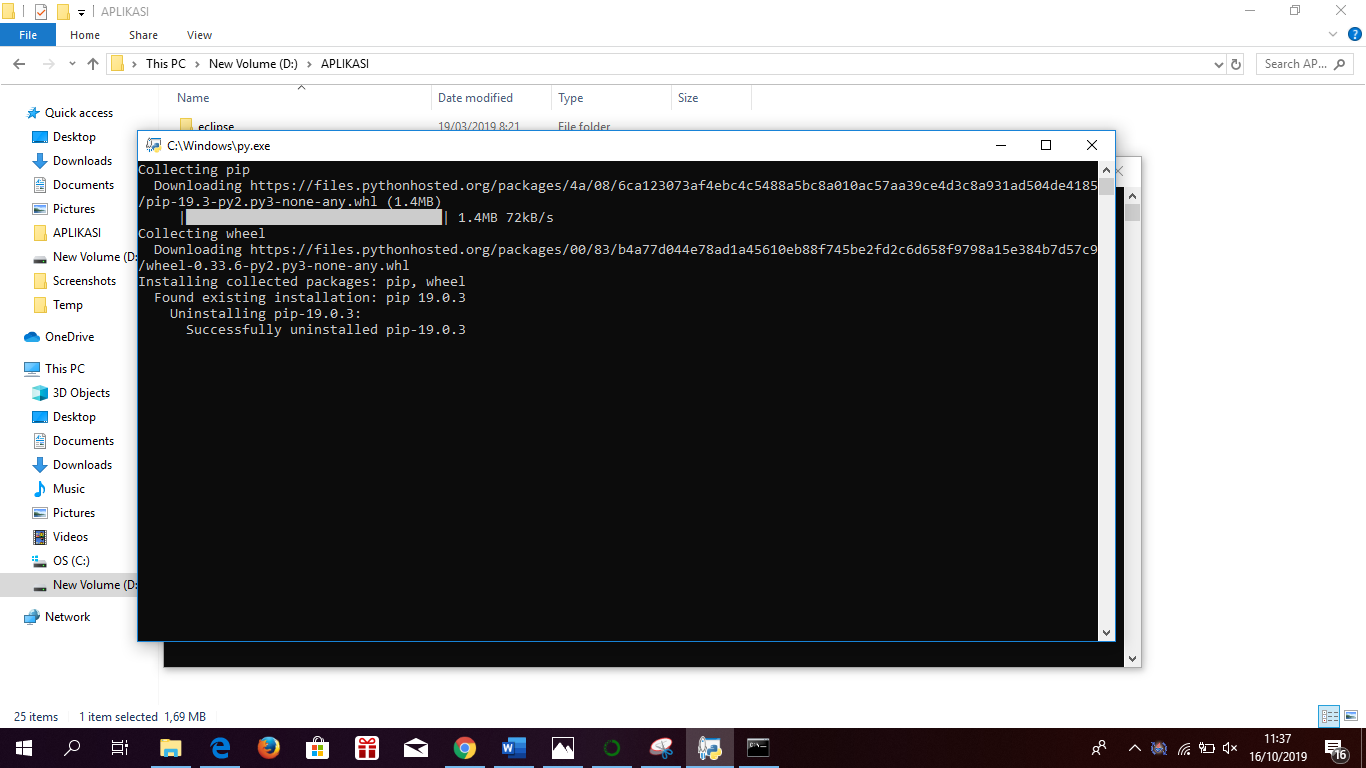
\includegraphics[scale=0.5]{figures/Screenshot (19).png}
            \caption{Caption}
            \label{fig:my_label}
        \end{figure}
    \end{itemize}
    \item cara setting environment
    \begin{itemize}
    \item buka control panel->system & sequrity->system 1.7
    \begin{figure}
    \centering
    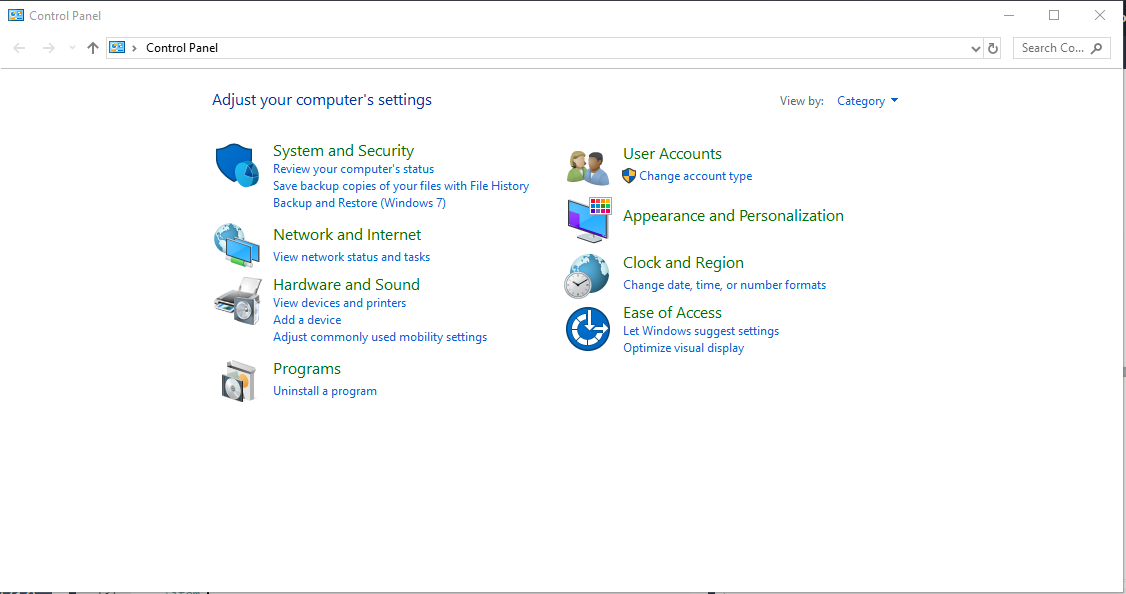
\includegraphics[scale=0.5]{figures/5.PNG}
        \caption{Caption}
        \label{fig:my_label}
    \end{figure}
        \item buka system properties->advance->environments variable 1.8
         \begin{figure}
    \centering
    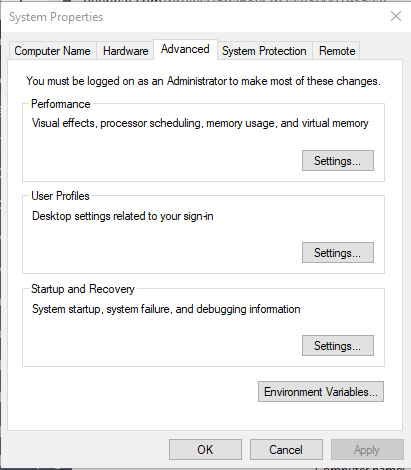
\includegraphics[scale=0.5]{figures/6.PNG}
        \caption{Caption}
        \label{fig:my_label}
    \end{figure}
        \item pada system variable klik dua kali pada path 1.9
         \begin{figure}
    \centering
    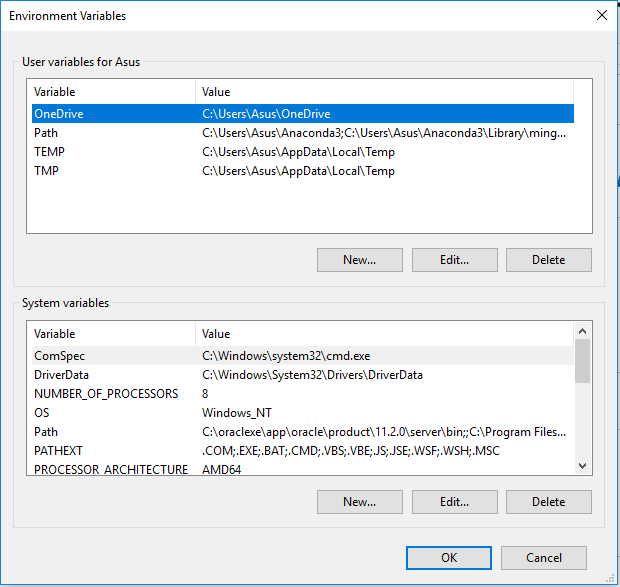
\includegraphics[scale=0.5]{figures/7.PNG}
        \caption{Caption}
        \label{fig:my_label}
    \end{figure}
        \item lalu tambahkan ;c:37 di yang paling atas lalu ok 1.10
         \begin{figure}
    \centering
    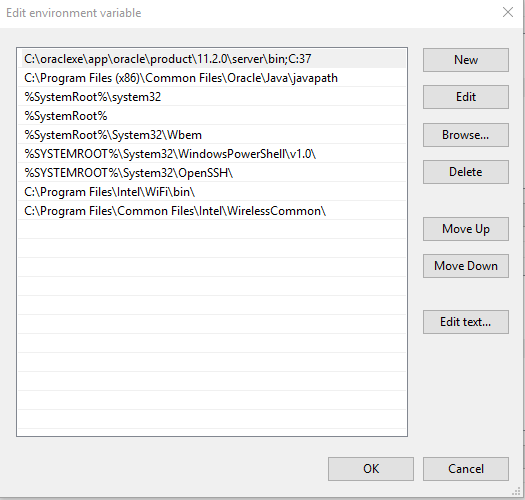
\includegraphics[scale=0.5]{figures/8.PNG}
        \caption{Caption}
        \label{fig:my_label}
    \end{figure}
        \item buka cmd dan tulis pip install request dan enter lalu tunggu 1.11 
         \begin{figure}
    \centering
    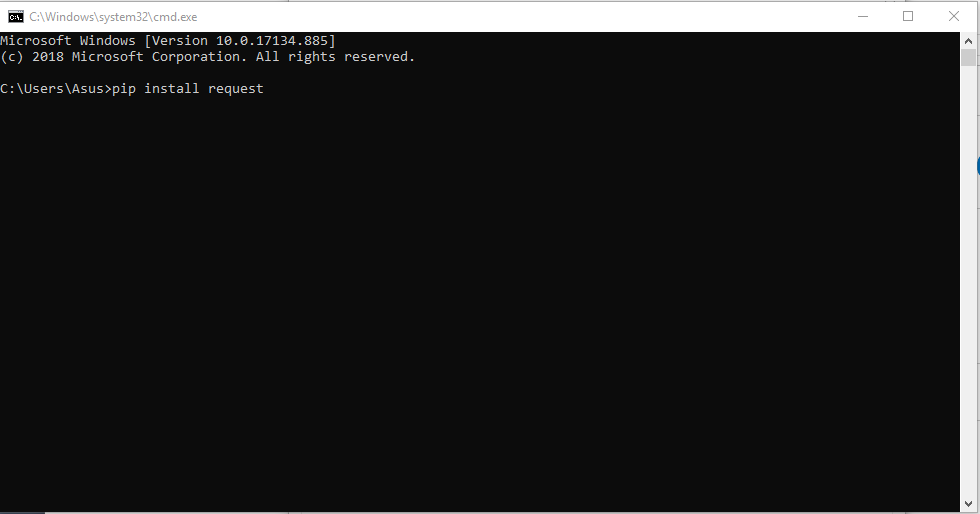
\includegraphics[scale=0.5]{figures/9.PNG}
        \caption{Caption}
        \label{fig:my_label}
    \end{figure}
        \item install berhasil 1.12
         \begin{figure}
    \centering
    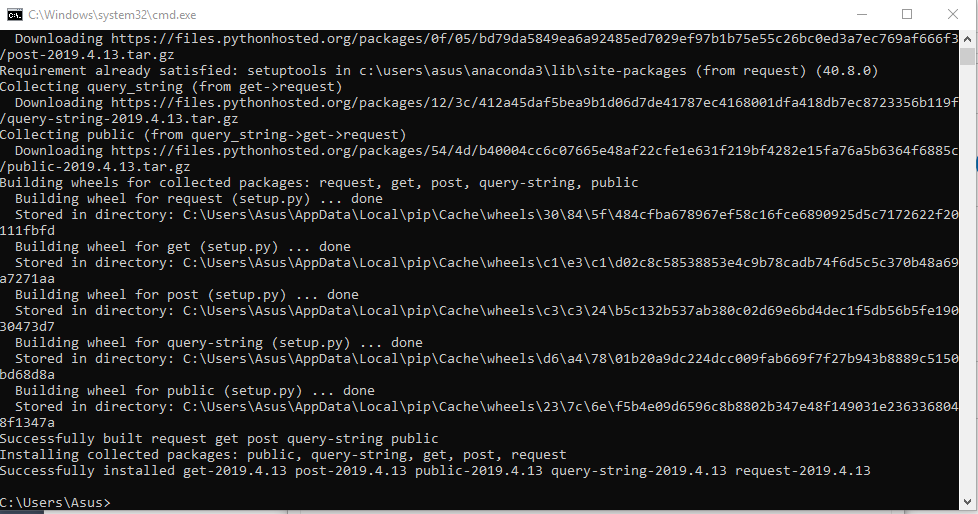
\includegraphics[scale=0.5]{figures/10.PNG}
        \caption{Caption}
        \label{fig:my_label}
    \end{figure}
    \end{itemize}
    \item mencoba entrepreter/cli melakui terminal atau cmd windows 
    \begin{itemize}
    \item buka cmd ->ketik pyhton->lalu ketik yang kita inginkan1.13
    \begin{figure}
    \centering
    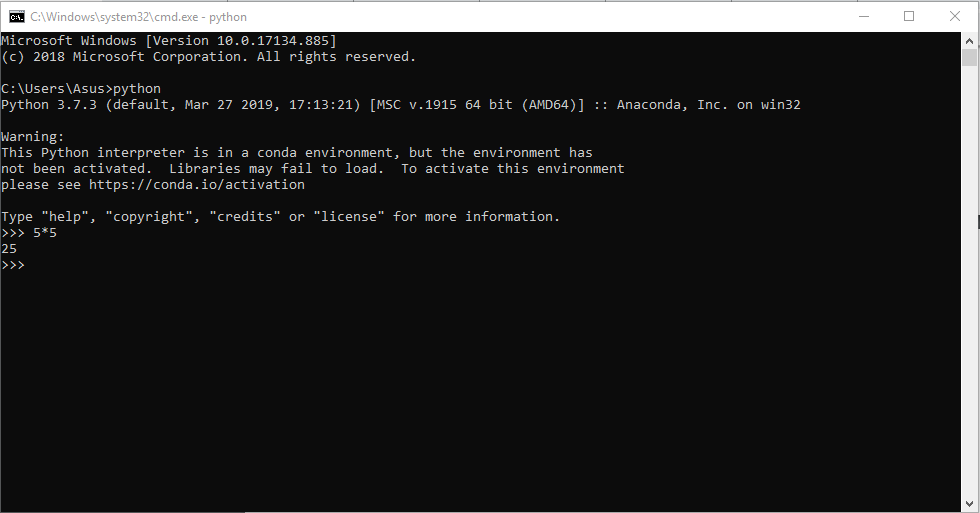
\includegraphics[scale=0.5]{figures/11.PNG}
        \caption{Caption}
        \label{fig:my_label}
    \end{figure}
    \end{itemize}
    \item Menjalankan dan mengupdate anaconda dan spyder
    \begin{itemize}
    \item buka anaconda navigator lalu launch pada spider 1.14
    \begin{figure}
    \centering
    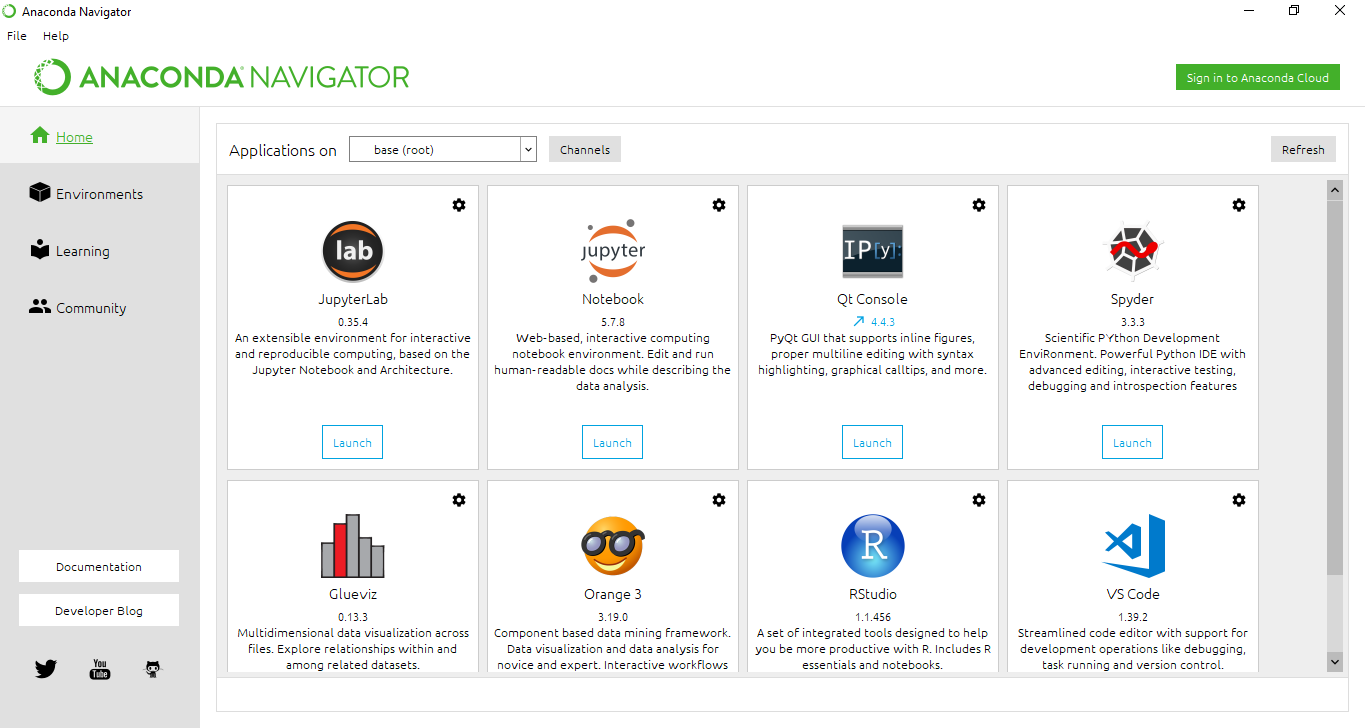
\includegraphics[scale=0.4]{figures/12.PNG}
        \caption{Caption}
        \label{fig:my_label}
    \end{figure}
    \end{itemize}
    \item Cara menjalankan Script hello world di spyder 
    \begin{itemize}
        \item buka aplikasi spider lalu tulis " print ("hello world") " 1.15
        \begin{figure}
    \centering
    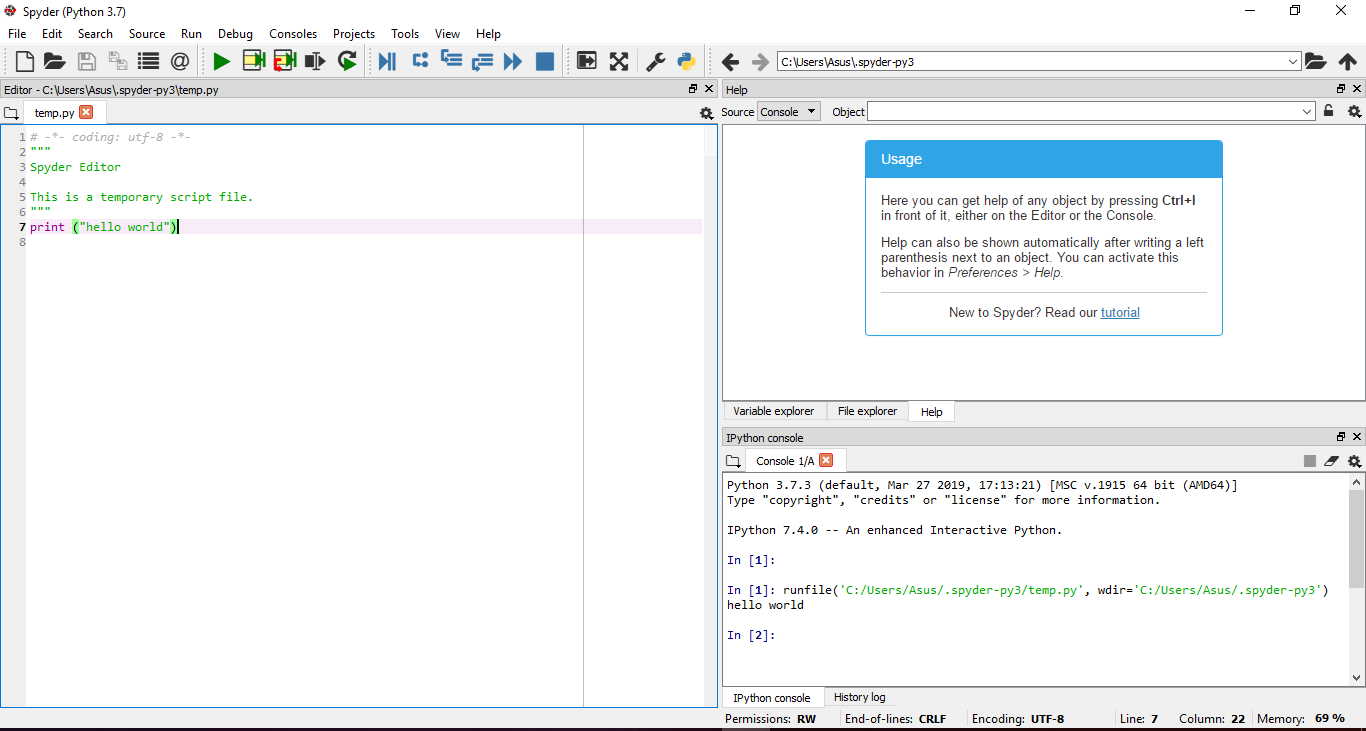
\includegraphics[scale=0.4]{figures/13.PNG}
        \caption{Caption}
        \label{fig:my_label}
    \end{figure}
    \end{itemize}
    \item Cara pemakaian variable explorer di spyder
    \begin{itemize}
    \item buka spyder lalu buat variabelnya seperti di contoh saya lalu di run 1.16
    \begin{figure}
    \centering
    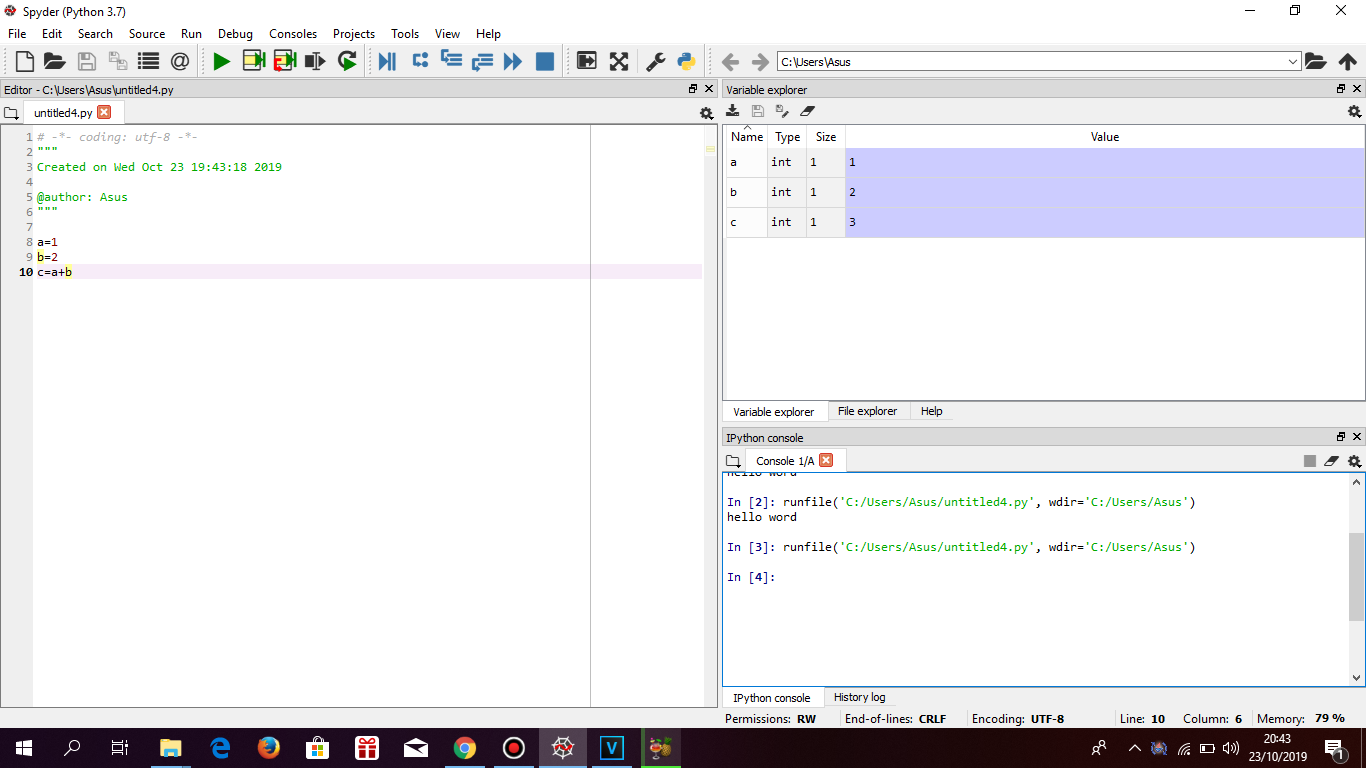
\includegraphics[scale=0.4]{figures/Screenshot (21).png}
        \caption{Caption}
        \label{fig:my_label}
    \end{figure}
    \end{itemize}
\end{enumerate}